


\section{Descripción del problema}
En la actualidad debido al crecimiento de personal calificado y graduado para tareas tecnológicas, las habilidades blandas o emocionales se han transformado en algo fundamental para el éxito profesional y personal, siendo estas las que permiten la interacción efectiva con los demás. Algunas de las habilidades blandas más demandadas por las empresas según los egresados universitarios son la proactividad, la capacidad de trabajo en equipo, la adaptabilidad, la inteligencia emocional y demás capacidades que ayudan a la toma de decisiones, solución de problemas e innovación de productos como se vio en el artículo de sobre Habilidades blandas y su importancia de aplicación en el entorno laboral.\cite{d}\\ \\

Estas habilidades consideradas fundamentales en la formación académica y laboral complementarias para el conocimiento técnico y científico son a menudo aquellas de las cuales no se recibe una adecuada educación durante los diferentes procesos de escolaridad. Los conocimientos más implementados durante la enseñanza en la universidad son de hecho los teóricos y prácticos, desestimando la importancia de competencias transversales que diversifiquen la aplicación del conocimiento en contextos reales. Esto a su vez genera una brecha entre los universitarios recién graduados y lo que en realidad se necesita en el mercado laboral.
\\ \\
En el caso específico de la ingeniería en sistemas, las habilidades blandas se vuelven aún más relevantes debido a la naturaleza colaborativa y multidisciplinaria del campo. Los ingenieros en sistemas no solo necesitan habilidades técnicas para diseñar, desarrollar e implementar soluciones tecnológicas, sino también competencias interpersonales que les permitan trabajar de manera eficiente en equipos y comunicarse con partes interesadas de diferentes niveles de experiencia técnica.
\\ \\
Estas habilidades son comúnmente solicitadas incluso de forma directa en diversos trabajos, un claro ejemplo ello se puede encontrar al usar aplicaciones enfocadas en la búsqueda de empleo como glassdoor el cual da decenas de miles de resultados para las soft skill o habilidades blandas en países como estados unidos o algunos cientos en países como el nuestro, como se demuestra a continuación:


\begin{figure}[ht]
  \centering
  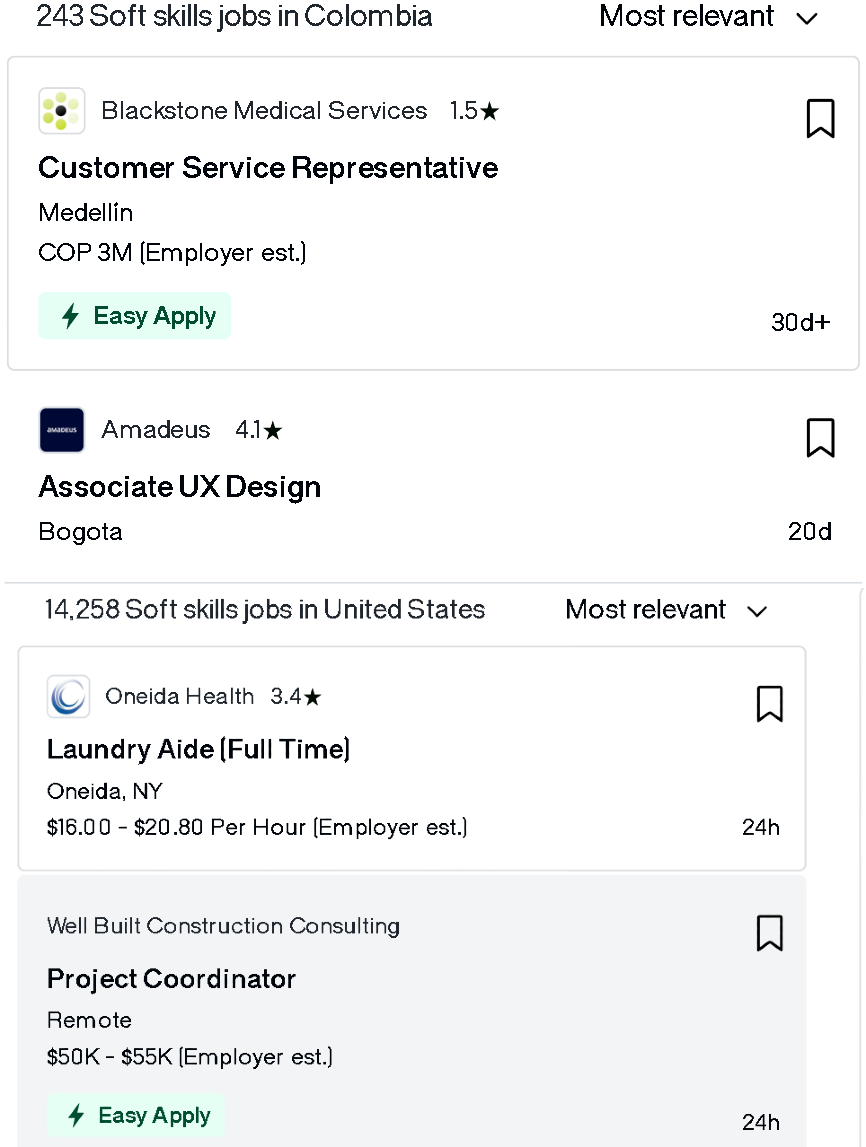
\includegraphics[width=0.5\linewidth]{Imagenes/glasdoor.png}
  \caption{Extraida de glasdoor\cite{q}}
  \label{fig:imagen}
\end{figure}
\newpage
Por consiguiente es necesario desarrollar las habilidades de los estudiantes de pregrado, para ello se puede optar por diferentes medios de educación como son el aprendizaje colaborativo que se basa formar un grupo con el objetivo aprender unos de otros, al discutir ideas y desarrollar habilidades sociales mientras resuelven problemas en conjunto o la gamificación la cual se refiere al uso y aplicación de mecánicas de juego en contextos no lúdicos la cual ha demostrado su eficacia en diferentes campos como la educación y la formación.
\\ \\
La gamificación en la educación tiene como objetivo principal transformar las experiencias de aprendizaje monótonas en actividades significativas y atractivas. Al integrar elementos de juegos en el proceso educativo, se busca motivar a los estudiantes a redescubrir la manera en que aprenden. Las clases que usan la gamificación están emergiendo como un método efectivo para comprometer a los estudiantes con un tema académico en particular. Este enfoque no solo reemplaza los métodos tradicionales, sino que también los mejora y revitaliza, ofreciendo una forma más dinámica de enseñanza.
\\ \\
La gamificación va más allá de simplemente otorgar puntos o premios en clase. Su verdadero potencial radica en convertir el entorno educativo en una experiencia divertida y enriquecedora, donde se exploran las pasiones y motivaciones de los estudiantes. Esta metodología permite comprender mejor a los alumnos, ya que un enfoque educativo desprovisto de elementos gamificados limita su participación activa. Integrar estrategias gamificadas no solo impulsa la participación estudiantil, sino que también crea un ambiente didáctico motivador, enriquecido con la emoción de la sorpresa y la gratificación.\cite{e}
\\ \\
Es verdad que, a pesar de la eficacia demostrada de estos métodos de enseñanza, a menudo enfrentan desafíos en términos de su disponibilidad y desarrollo centralizado en plataformas accesibles para su uso generalizado.
\section{Formulación del problema}
En consecuencia en búsqueda de describir el problema  y hallar una idea más clara se llega al siguiente interrogante.
\\ \\
¿Cuál sería la metodología para el diseño y la gamificación de dos módulos centrados en las habilidades 'fitness' y 'mindset' destinados a ser integrados en un prototipo de plataforma web?